% **************************************************************
% Hi! Edit this file for your presentation!
% **************************************************************

% ==================///==================///==================///
% ==================/// LATEX'S STUFF
% ==================///==================///==================///

\documentclass{beamer}
\usepackage{amsfonts,amsmath,oldgerm}
\usepackage{listings}
\usepackage{graphics,graphicx}
\usepackage{mdframed} 
\usetheme{_statale}
\usefonttheme[onlymath]{serif}

\lstdefinestyle{statalepython}{
    language=Python,
    backgroundcolor=\color{statalegray},
    basicstyle=\scriptsize\ttfamily,
    keywordstyle=\color{maincolor}\bfseries,
    stringstyle=\color{statalegreen},
    commentstyle=\color{stataledarkgreen}\itshape,
    numberstyle=\tiny\color{gray},
    numbers=none,
    numbersep=8pt,
    stepnumber=1,
    showstringspaces=false,
    breaklines=true,
    frame=single,
    tabsize=4,
    captionpos=b
}

\newcommand{\testcolor}[1]{\colorbox{#1}{\textcolor{#1}{test}}~\texttt{#1}}
\newcommand{\hrefcol}[2]{\textcolor{cyan}{\href{#1}{#2}}}
\titlebackground*{assets/background}

% ==================///==================///==================///
% ==================/// SPLASH PAGE
% ==================///==================///==================///

\title{Verifiche di compliance in ambienti Cloud}
\subtitle{Presentazione dell'elaborato finale}
\course{Laurea Triennale in Sicurezza dei Sistemi e delle Reti Informatiche}
\author{\href{mailto:niccolo.volonte@studenti.unimi.it}{Niccolò Volontè}}
\IDnumber{20642A}
\date{16 luglio 2025}

% ==================///==================///==================///
% ==================///  START PRESENTATION
% ==================///==================///==================///

\begin{document}
\maketitle

\footlinecolor{maincolor}


% ==================///==================///==================///
% ==================/// BODY'S PRESENTATION
% ==================///==================///==================///

\begin{frame}{Introduzione e obiettivi}
    \framesubtitle{Contesto e finalità}
    \begin{itemize}
        \item Evoluzione del Cloud Computing e modelli (IaaS, PaaS, SaaS)
        \item AWS come contesto di riferimento
        \item La compliance come sfida attuale
        \item Sviluppo di sonde per verificare la compliance in ambienti Cloud
        \item Integrazione nella piattaforma Moon Cloud
    \end{itemize}
\end{frame}


\begin{frame}{Compliance e standard nel cloud}
    \framesubtitle{Significato, sfide e riferimenti normativi}
    \begin{columns}
        \begin{column}{0.6\textwidth}
            \begin{itemize}
                \item \textbf{Compliance:} rispetto di requisiti normativi e di sicurezza
                \item Importanza crescente nel contesto cloud
                \item Sfide legate alla gestione di risorse distribuite
                \item \textbf{Standard} di riferimento:
                \begin{itemize}
                    \item Center for Internet Security (\emph{CIS}) - \hrefcol{https://www.cisecurity.org/}{CIS AWS Foundations Benchmark}
                    \item National Institute of Standards and Technology (\emph{NIST}) - \hrefcol{https://www.nist.gov/}{NIST SP 800-53}
                \end{itemize}
            \end{itemize}
        \end{column}
        \begin{column}{0.4\textwidth}
            
\includegraphics[width=\textwidth]{assets/cisnist.png}
        \end{column}
    \end{columns}
\end{frame}


\begin{frame}{Standard di riferimento}
    \framesubtitle{Esempio di controllo per \texttt{aws\_account}}
    \begin{mdframed}[backgroundcolor=statalegrey]
    \textbf{1.4 Ensure MFA is enabled for the 'root' user account (Automated)}
    \begin{itemize}
        \item \textbf{Profile Applicability:} Level 1
        \item \textbf{Description:} The 'root' user account is the most privileged user in an AWS account. Multi-factor Authentication (MFA) adds an extra layer of protection on top of a username and password. With MFA enabled, when a user signs in to an AWS website, they will be prompted for their username and password as well as for an authentication code from their AWS MFA device.
        \item \textbf{Rationale:} Enabling MFA provides increased security for console access as it requires the authenticating principal to possess a device that emits a time-sensitive key and have knowledge of a credential.
    \end{itemize} 
\end{mdframed}
\end{frame}

\begin{frame}{Tecnologie utilizzate}
    \framesubtitle{Linguaggi e strumenti}
    \begin{columns}
        \begin{column}{0.4\textwidth}
            \begin{itemize}
                \item \emph{Python} come linguaggio di programmazione
                \item \texttt{Boto3} per l'interazione con AWS
                \item \emph{Moon Cloud} come piattaforma di integrazione
            \end{itemize}
        \end{column}
        \begin{column}{0.6\textwidth}
            \begin{colorblock}[black]{statalegrey}{Esempio di utilizzo di Boto3}
                \texttt{\textcolor{maincolor}{import} boto3}\\
                \texttt{client = boto3.\textcolor{maincolor}{client}(}\\
                \texttt{    \textcolor{statalegreen}{'sqs'},}\\
                \texttt{    region\_name=\textcolor{statalegreen}{'eu-central-1'},}\\
                \texttt{    aws\_access\_key\_id=\textcolor{statalegreen}{'YOUR\_ACCESS\_KEY'},}\\
                \texttt{    aws\_secret\_access\_key=\textcolor{statalegreen}{'YOUR\_SECRET\_KEY'}}\\
                \texttt{)}\\
                \texttt{response = client.\textcolor{maincolor}{list\_queues}()}\\
            \end{colorblock}
        \end{column}
    \end{columns}
\end{frame}

\begin{frame}{Moon Cloud}
    \framesubtitle{Piattaforma, funzionalità e architettura}
    \begin{columns}
        \begin{column}{0.7\textwidth}
            \begin{itemize}
                \item Esegue sonde di assurance su infrastrutture ICT
                \item Architettura basata su immagini Docker e CI/CD
                \item Dashboard per la gestione dei target, credenziali e risultati
                \item Modello a stati finiti: \textit{forward}, \textit{rollback}
            \end{itemize}
        \end{column}
        \begin{column}{0.3\textwidth}
            
\includegraphics[width=\textwidth]{assets/mooncloud.png}
        \end{column}
    \end{columns}
\end{frame}

\begin{frame}{Struttura di una sonda}
    \framesubtitle{Componenti per la creazione}
    \begin{columns}
        \begin{column}{0.6\textwidth}
            \begin{itemize}
                \item Codice Python all'interno del file \texttt{probe.py}
                \item \texttt{schema.json} e \texttt{test.json} per input validato
                \item \texttt{Dockerfile}, \texttt{.gitlab-ci.yml} per la pipeline
                \item Struttura con \texttt{atoms} eseguiti in sequenza
                \item Output \emph{strutturato}
            \end{itemize}
        \end{column}
        \begin{column}{0.4\textwidth}
            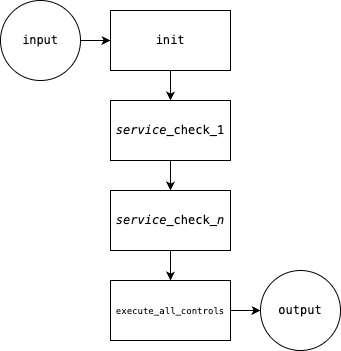
\includegraphics[width=\textwidth]{assets/flow.drawio.png}
        \end{column}
    \end{columns}
\end{frame}

% \begin{frame}{Esempio di sonda}
%     \framesubtitle{Sonda \texttt{aws\_sqs}}
%     \begin{columns}
%         \begin{column}{0.4\textwidth}
%             \begin{itemize}
%                 \item Controlli relativi a crittografia, tagging, policy pubbliche
%                 \item Basata su controlli di AWS Security Hub
%                 \item Esempio di scansione multiregione
%                 \item Integra parametri personalizzati via dashboard
%             \end{itemize}
%         \end{column}
%         \begin{column}{0.6\textwidth}
%             \begin{colorblock}[black]{statalegrey}{Implementazione multiregione}
%                 \texttt{\textcolor{maincolor}{self}.clients = \string{\string}}\\
%                 \texttt{\textcolor{maincolor}{for} idx, region in \textcolor{maincolor}{enumerate}(specific\_regions, start=1):}\\
%                     \texttt{    \textcolor{maincolor}{self}.clients[\textcolor{statalegreen}{f'client\_\string{idx\string}'}] = \textcolor{maincolor}{boto3}.client(}\\
%                     \texttt{    \textcolor{statalegreen}{'sqs'},}\\
%                     \texttt{    aws\_access\_key\_id=\textcolor{statalegreen}{'YOUR\_ACCESS\_KEY'},}\\
%                     \texttt{    aws\_secret\_access\_key=\textcolor{statalegreen}{'YOUR\_SECRET\_KEY'}}\\
%                     \texttt{    region\_name=\textcolor{statalegreen}{'eu-central-1'},}\\
%                     \texttt{)}\\
%             \end{colorblock}
%         \end{column}
%     \end{columns}
% \end{frame}

\begin{frame}[fragile]{Esempio: \texttt{aws\_sqs}}
\framesubtitle{Controllo cifratura, tag e accesso pubblico}
\begin{itemize}
    \item Controlli relativi a crittografia, tagging, e policy pubbliche
    \item Integra scansione multiregione
    \item Ogni controllo è una funzione separata
\end{itemize}

\vspace{0.3cm}
\textbf{Snippet: gestione client multiregione e controllo SQS.1}
\begin{lstlisting}[style=statalepython, basicstyle=\scriptsize\ttfamily]
specific_regions = re.split(r'[,;\s]+', raw_regions) if raw_regions else []
for idx, region in enumerate(specific_regions[:6], start=1):
    self.clients[f'client_{idx}'] = boto3.client(...)
# ... sqs_check_1 ...
attr_response = client.get_queue_attributes(
    AttributeNames=['SqsManagedSseEnabled'],
    QueueUrl=queue_url
)
if attr_response.get('Attributes', {}).get('SqsManagedSseEnabled') == 'true':
    encrypted_queues.append(...)
else unencrypted_queues.append(...)
\end{lstlisting}
\end{frame}


\begin{frame}{\texttt{aws\_vulnerability}}
    \framesubtitle{Sonda per la gestione CVE}
    \begin{columns}
        \begin{column}{0.4\textwidth}
            \begin{itemize}
            \item Sonda custom che elenca CVE trovate da AWS Inspector
            \item Analisi di Elastic Container Registry (\emph{ECR}), 
                Elastic Compute Cloud (\emph{EC2}) e \emph{Lambda} functions
            \item Consente una visione dinamica del rischio
        \end{itemize}
        \end{column}
        \begin{column}{0.6\textwidth}
            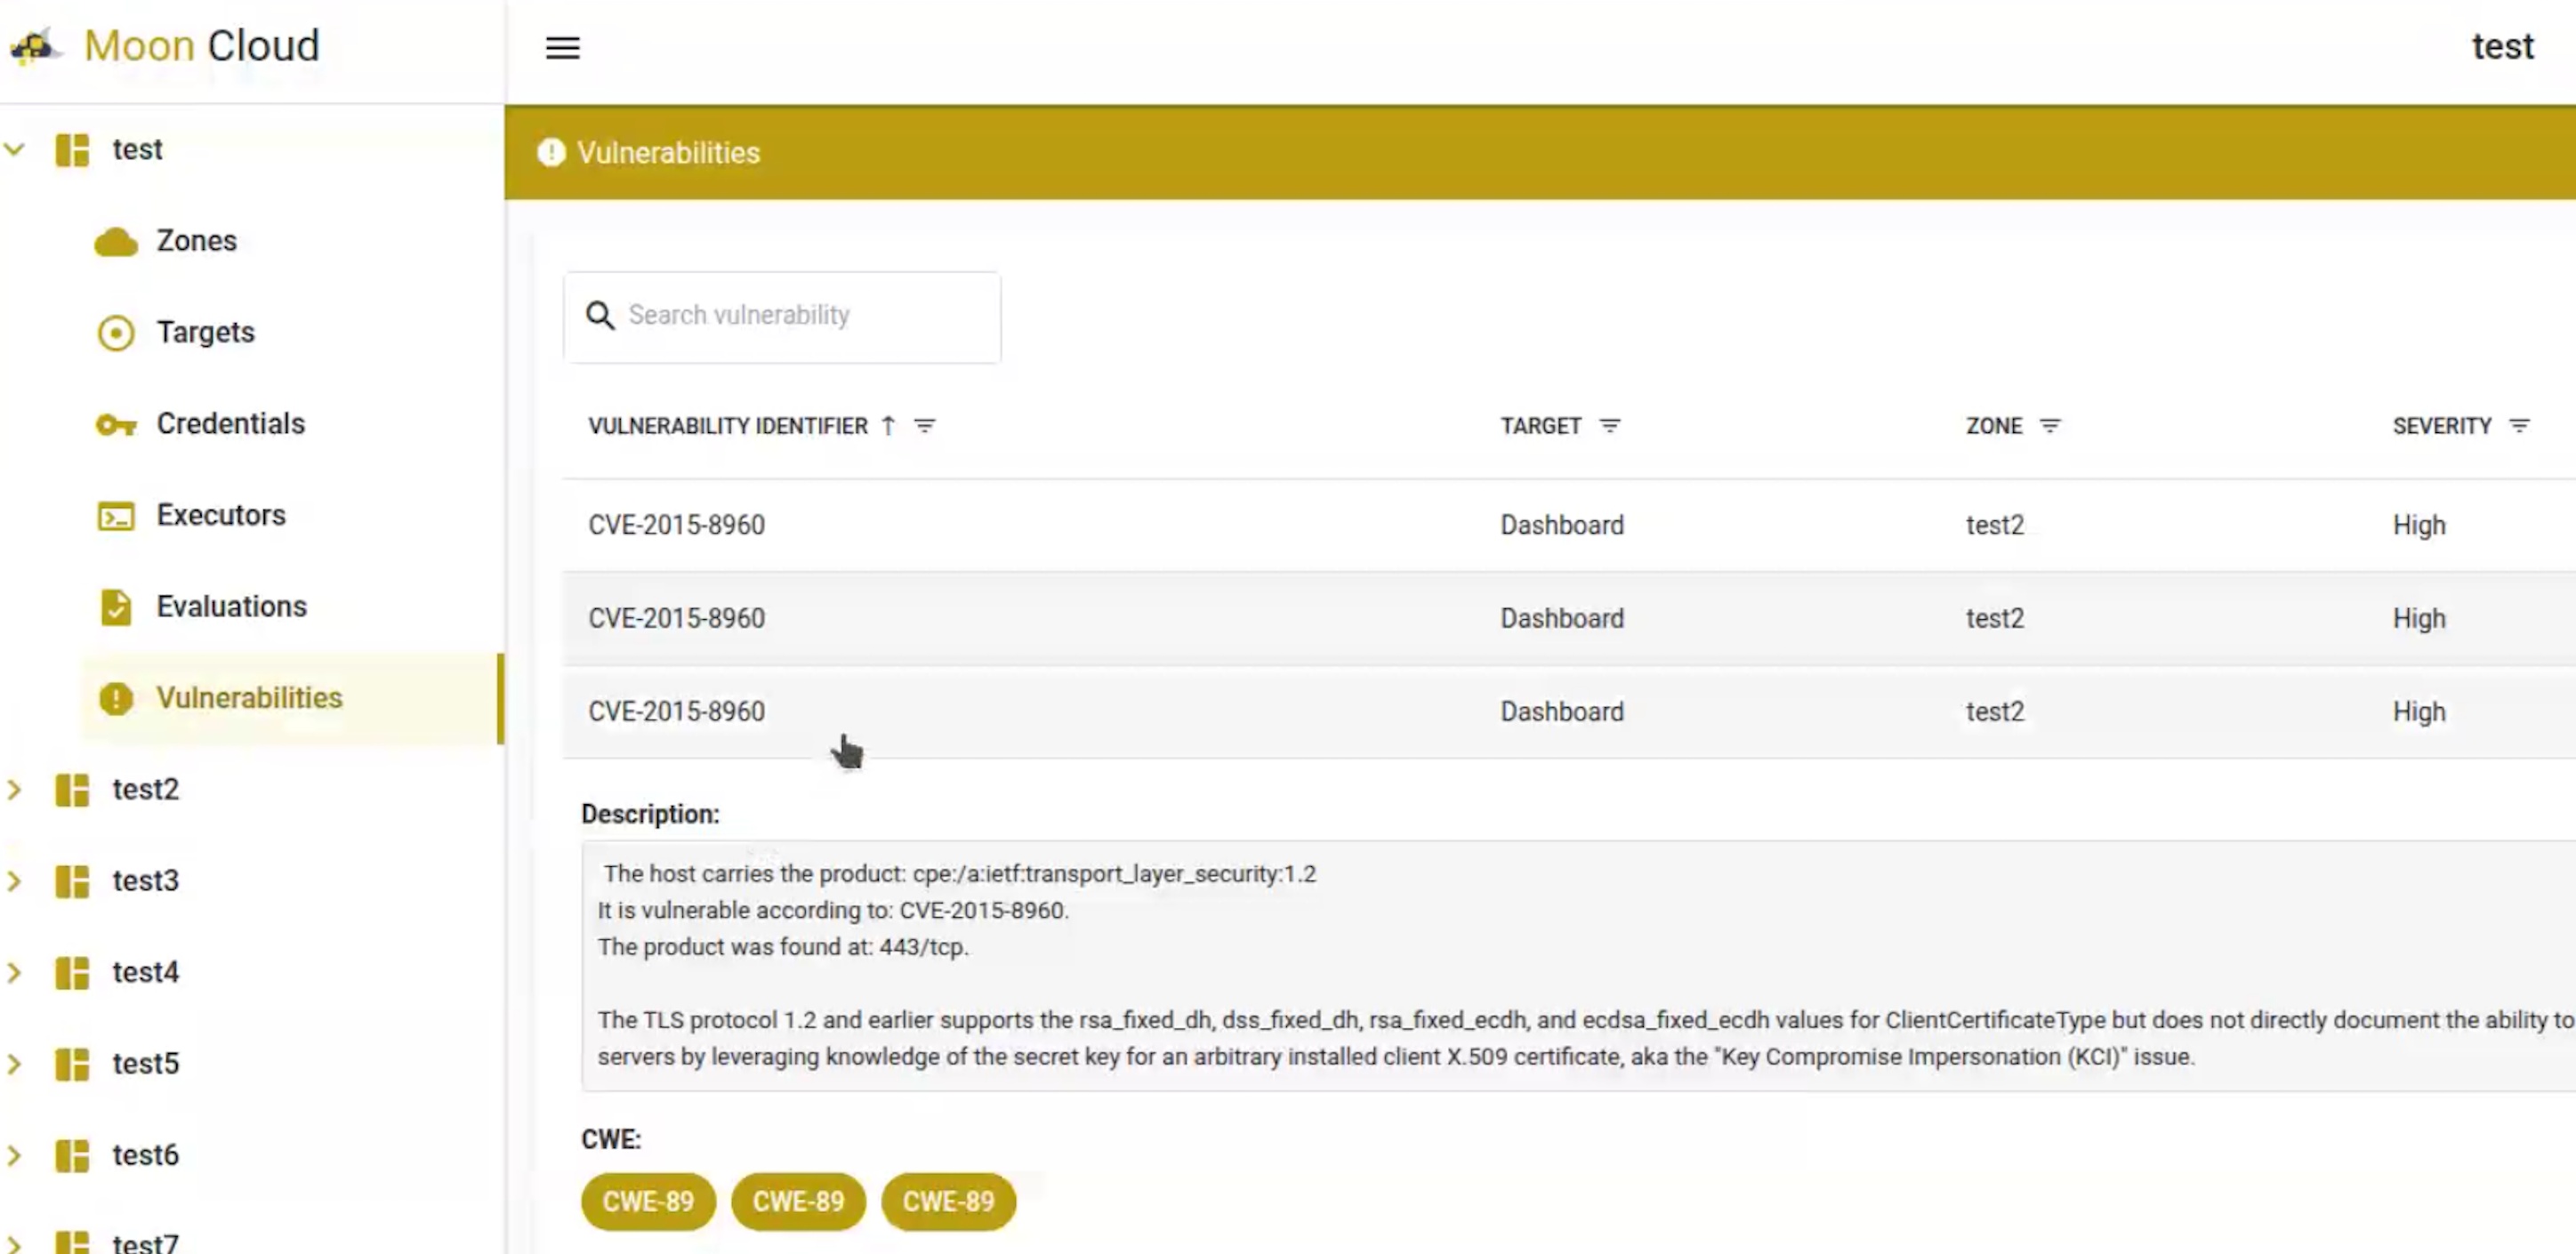
\includegraphics[width=\textwidth]{assets/Screenshot 2025-07-08 at 10.56.53.png}
        \end{column}
    \end{columns}
\end{frame}

\begin{frame}{Deploy e output delle sonde}
    \framesubtitle{Esecuzione, integrazione e risultati}
    \begin{columns}
        \begin{column}{0.5\textwidth}
            \textbf{Esecuzione e integrazione}
            \begin{itemize}
                \item Pipeline CI/CD su GitLab per ogni sonda
                \item Input via JSON schema con validazione
                \item Gestione delle credenziali
                \item Integrazione nel backend di Moon Cloud
            \end{itemize}
        \end{column}
        \begin{column}{0.5\textwidth}
            \textbf{Risultati ottenuti}
            \begin{itemize}
                \item Controlli strutturati in blocchi
                \item Risultato numerico e descrittivo
                \item Sommario con percentuale di conformità
                \item Log dettagliato con eccezioni gestite
            \end{itemize}
        \end{column}
    \end{columns}
\end{frame}


\begin{frame}{Competenze acquisite e sviluppi futuri}
    \framesubtitle{Riflessioni e prospettive}
    \begin{columns}
        \begin{column}{0.5\textwidth}
            \textbf{Competenze acquisite}
            \begin{itemize}
                \item Python, AWS, Docker, GitLab CI/CD                \item Analisi di documentazione tecnica
                \item Sviluppo modulare su un framework esistente
                \item Esperienza su progetto reale (Moon Cloud)
            \end{itemize}
        \end{column}
        \begin{column}{0.5\textwidth}
            \textbf{Sviluppi futuri}
            \begin{itemize}
                \item Estensione a nuovi benchmark e servizi AWS
                \item Apertura verso altri cloud provider
                \item Supporto multi regione
            \end{itemize}
        \end{column}
    \end{columns}
\end{frame}



% ==================///==================///==================///
% ==================/// END PRESENTATION
% ==================///==================///==================///

\backmatter
\end{document}